\documentclass[handout]{beamer}
\usepackage[spanish]{babel}
\usepackage[utf8]{inputenc}
\usepackage{graphicx}
\usepackage{multimedia}
\usepackage{animate}
\usepackage{tcolorbox}
\usepackage{newfloat}
\usepackage[version=4]{mhchem}


\usebackgroundtemplate{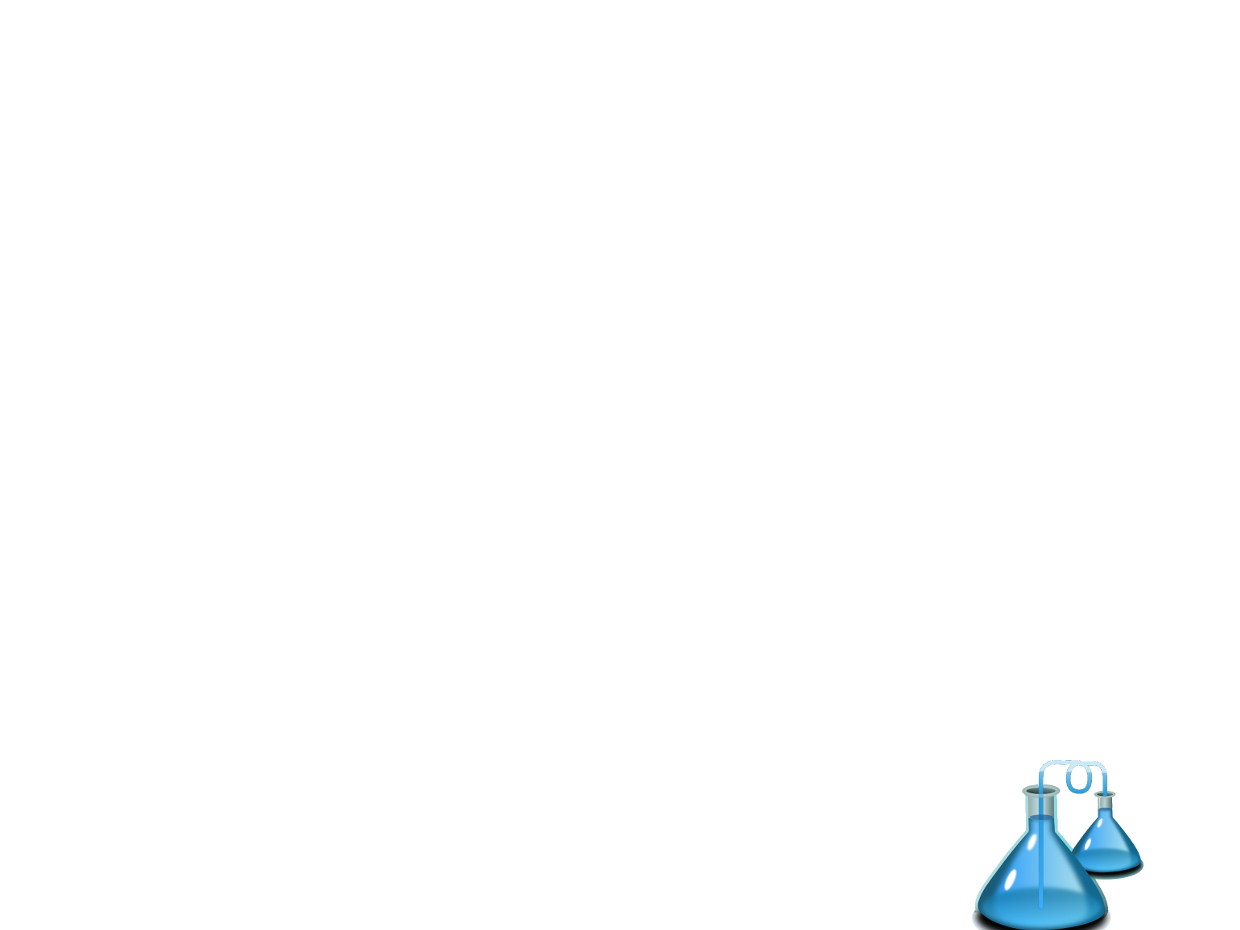
\includegraphics[width=\paperwidth]{template_2.jpg}}
\usefonttheme{structuresmallcapsserif}
\setbeamertemplate{footline}[frame number]
\setbeamertemplate{caption}[numbered]
\usepackage{wrapfig}
\usepackage{subcaption}

\usepackage[backend=bibtex, style=chem-acs]{biblatex}
\bibliography{../Mesoporosos}


\newrobustcmd*{\footfullcitenomark}{%
	\AtNextCite{%
		\let\thefootnote\relax
		\let\mkbibfootnote\mkbibfootnotetext}%
	\footfullcite}

\DeclareFloatingEnvironment[fileext=los, listname=Lista de Esquemas, name=Esquema, placement=tbhp]{scheme}

\begin{document}
{
	\usebackgroundtemplate{
\includegraphics[width=\paperwidth]{template.jpg}}
	\begin{frame}
	
		\centering
		\textsc{\LARGE S\'intesis de un material mesoporoso: SBA-15}
		\\
		\vspace{5cm}
		Juan Barbosa
	\end{frame}
}

\begin{frame}{Introducci\'on}
	\textbf{Definiciones}
	\begin{enumerate}
		\item \textbf{Materiales mesoporosos}: material que contiene poros de diametro entre 2 y 50 nm\footfullcitenomark{macnaught_wilkinson_1997}.
		\item \textbf{Copol\'imeros tribloque}
		\begin{figure}[h]
			\centering
			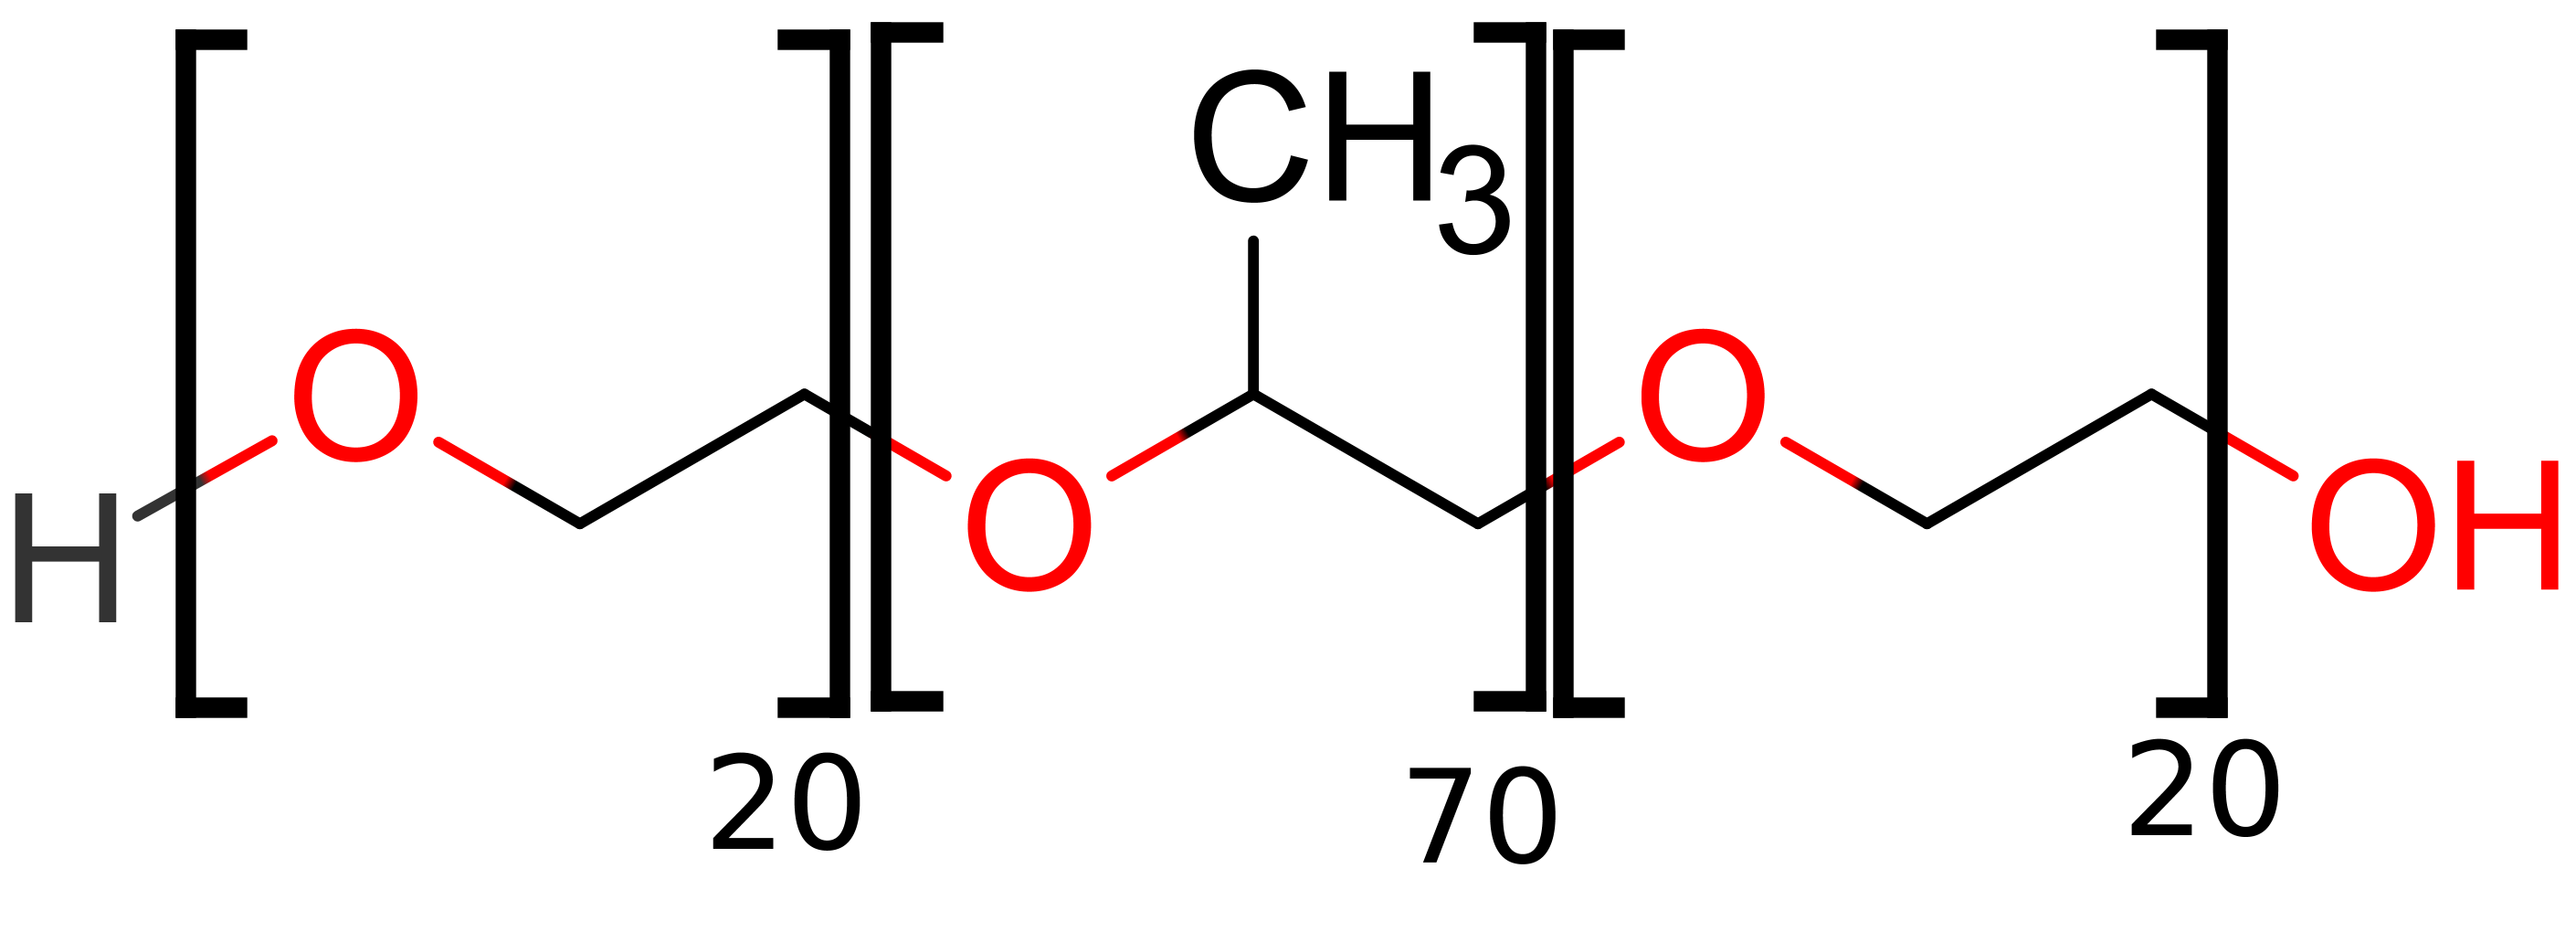
\includegraphics[width=0.5\linewidth]{../structures/Pluronic.png}
		\end{figure}
	\end{enumerate}
\end{frame}
\begin{frame}{Introducci\'on}
	\begin{columns}
		\begin{column}{0.5\linewidth}
			Los s\'olidos porosos son de utilidad en:
			\begin{itemize}
				\item Aplicaciones \'opticas
				\item Intercambio ionico
				\item Cat\'alisis
				\item Adsorci\'on
				\item Transporte de medicamentos
			\end{itemize}
		\end{column}
		\begin{column}{0.5\textwidth}
			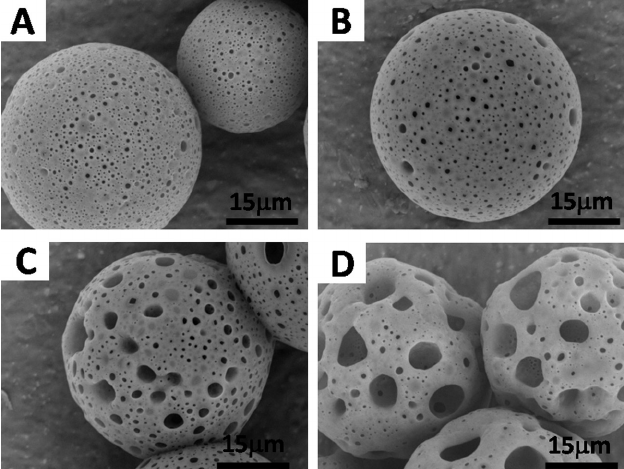
\includegraphics[width=\linewidth]{poros.png}
		\end{column}
	\end{columns}
	\footfullcitenomark{zhao_1998}
	\footfullcitenomark{vargas_legnoverde_giraldo_basaldella_moreno-pirajan_2010}
\end{frame}
\begin{frame}{SBA-15}
	Tipo de material Amorfo Santa Barbara, sintetizado por Zhao en la Universidad de California en Santa Barbara.
	\begin{itemize}
		\item Canales hexagonales
		\item Poros con diametros de 5 a 30 nm
		\item Grosor de las paredes de 0.5 - 2.0 nm
		\item Cilindros de 1 - 3 $\mu$m
	\end{itemize}
	\centering
	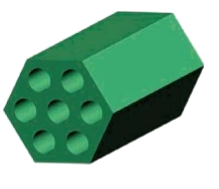
\includegraphics[width=0.3\linewidth]{sba-15.png}
	\footfullcitenomark{zhao_1998}
	\footfullcitenomark{zhao_huo_feng_chmelka_stucky_1998}
	\footfullcitenomark{vargas_legnoverde_giraldo_basaldella_moreno-pirajan_2010}
\end{frame}

\begin{frame}{Procedimiento experimental}
	\begin{columns}
		\begin{column}{0.5\textwidth}
			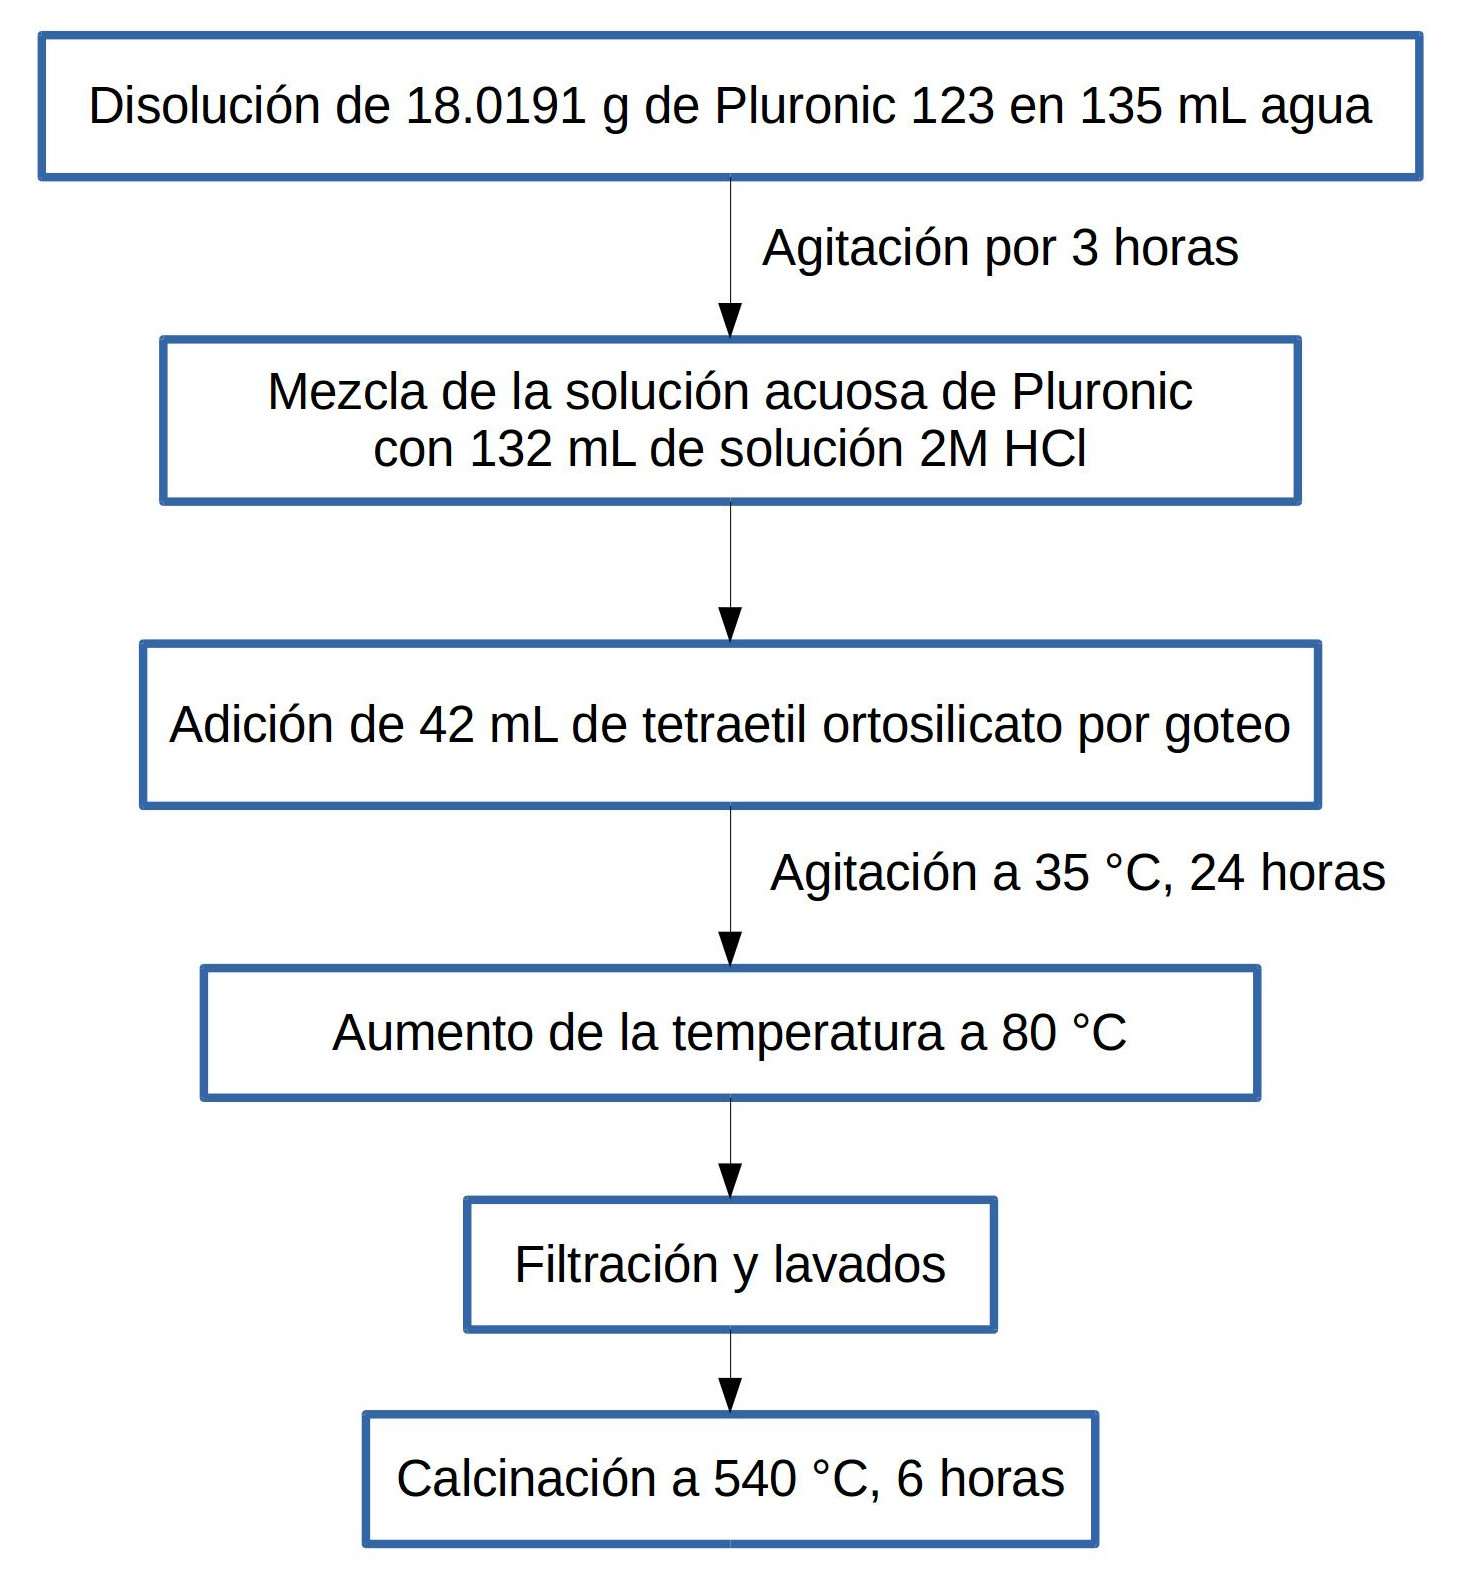
\includegraphics[width=\linewidth]{experimental1.jpg}
		\end{column}
		\begin{column}{0.5\textwidth}
			{\raggedright
			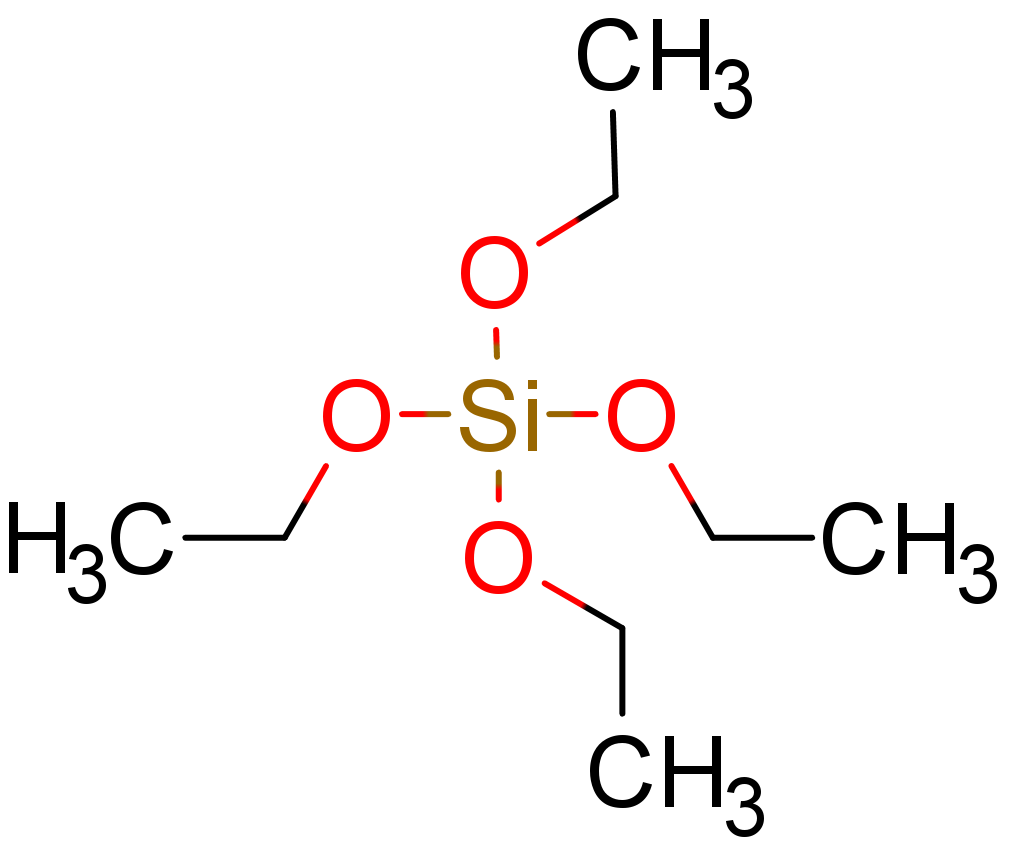
\includegraphics[width=0.5\linewidth]{../structures/silicate.png}
			
			Tetraetil ortosilicato
			}
		\end{column}
	\end{columns}
	
	\footfullcitenomark{zhao_1998}
\end{frame}

\begin{frame}{Procedimiento experimental}
	\begin{columns}
		\begin{column}{0.5\textwidth}
			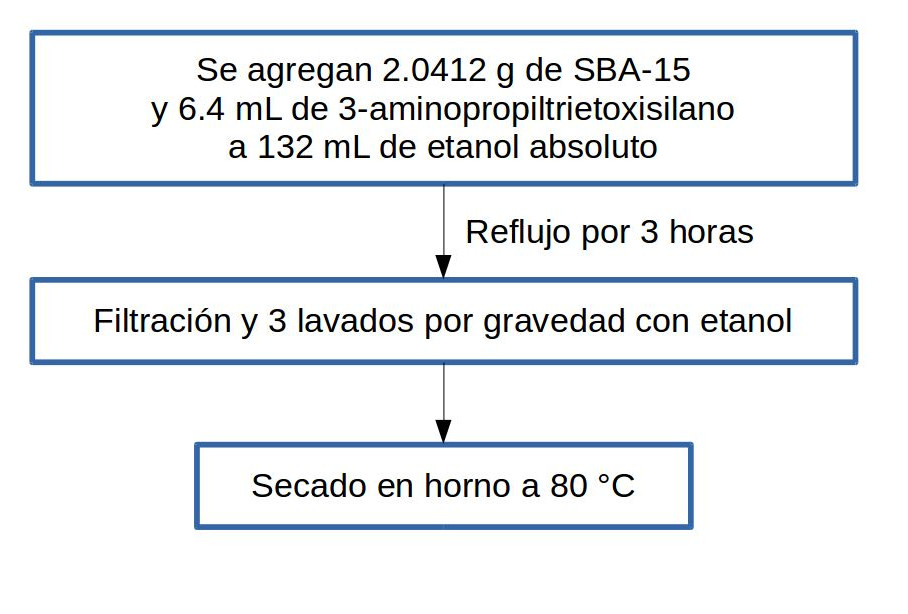
\includegraphics[width=\linewidth]{experimental2.jpg}
		\end{column}
		\begin{column}{0.5\textwidth}
			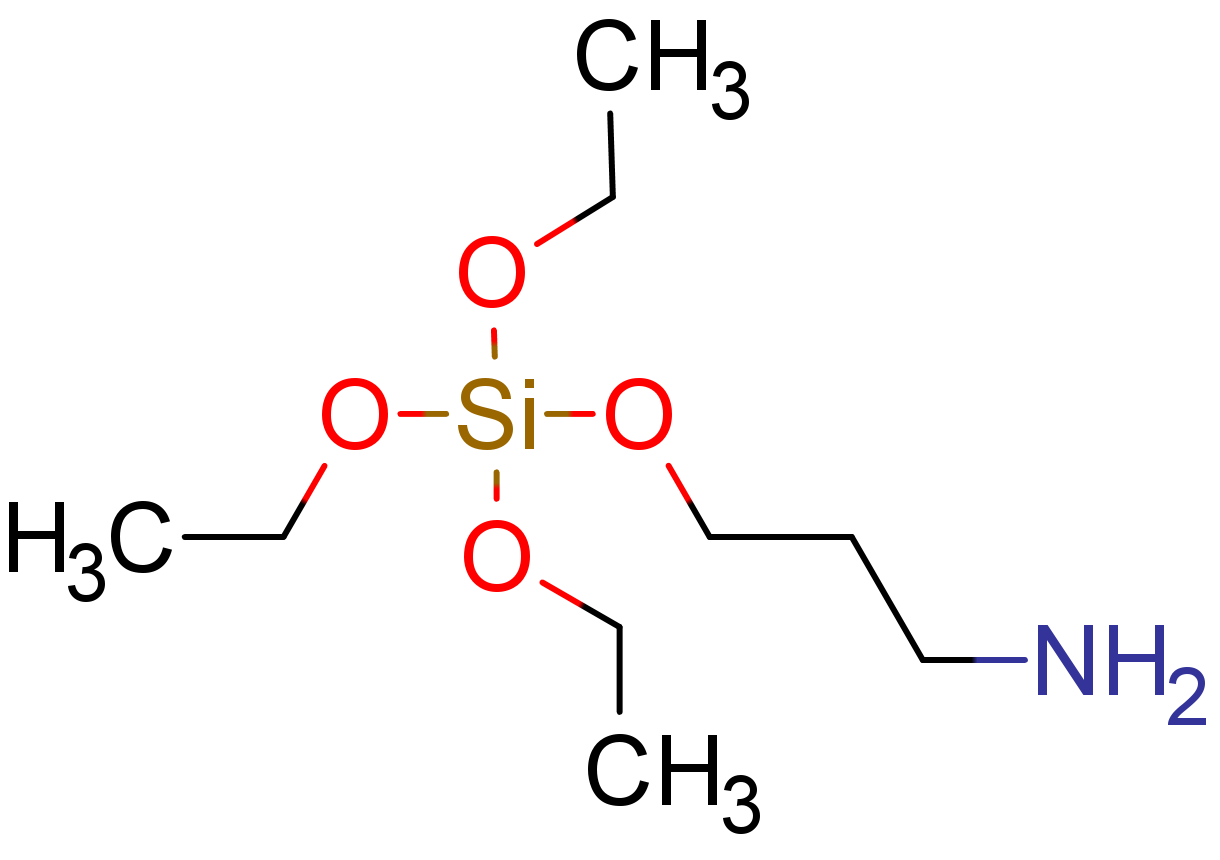
\includegraphics[width=0.5\linewidth]{../structures/aminosilicate.png}
			
			3-aminopropiltrietoxisilano (APTES)
		\end{column}
	\end{columns}
\end{frame}

\begin{frame}{Resultados}
	\textbf{An\'alisis termogravim\'etrico}
	\begin{columns}
		\begin{column}{0.5\textwidth}
			\begin{figure}
				\centering
				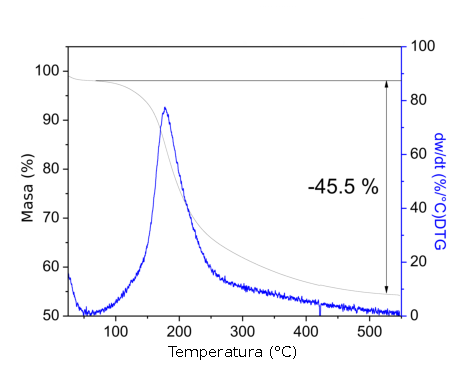
\includegraphics[width=\linewidth]{../structures/TGA-calcination.pdf}
				\caption{SBA-15.}
			\end{figure}
		\end{column}
		\begin{column}{0.5\textwidth}
			\begin{figure}
				\centering
				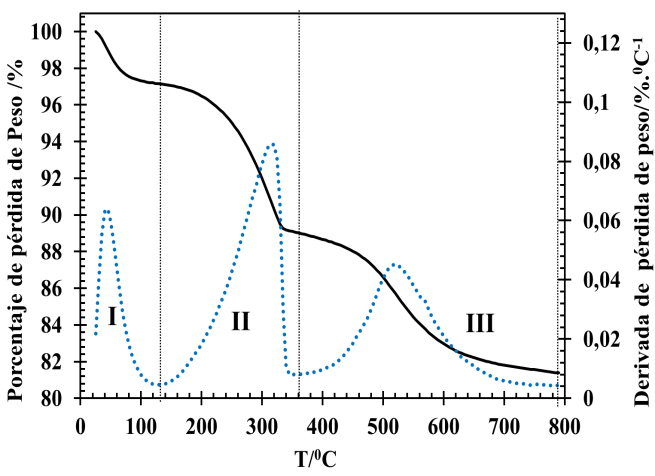
\includegraphics[width=\linewidth]{../structures/TGA-NH2.png}
				\caption{SBA-15-\ce{NH2}}
			\end{figure}
		\end{column}
	\end{columns}
	\footfullcitenomark{melendez_murillo_ramirez_2016}
	\footfullcitenomark{rodriguez}
\end{frame}

\begin{frame}{Resultados}
	\begin{columns}
		\begin{column}{0.5\textwidth}
			\begin{figure}
				\centering
				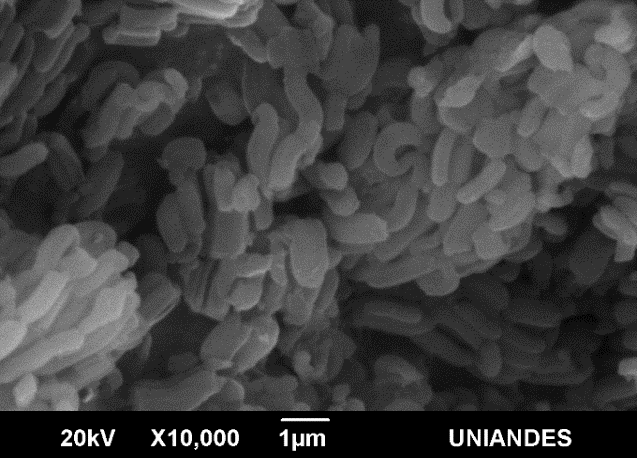
\includegraphics[width=\linewidth]{../structures/SEM.png}
				\caption{SEM.}
			\end{figure}
		\end{column}
		\begin{column}{0.5\textwidth}
			\begin{figure}
				\centering
				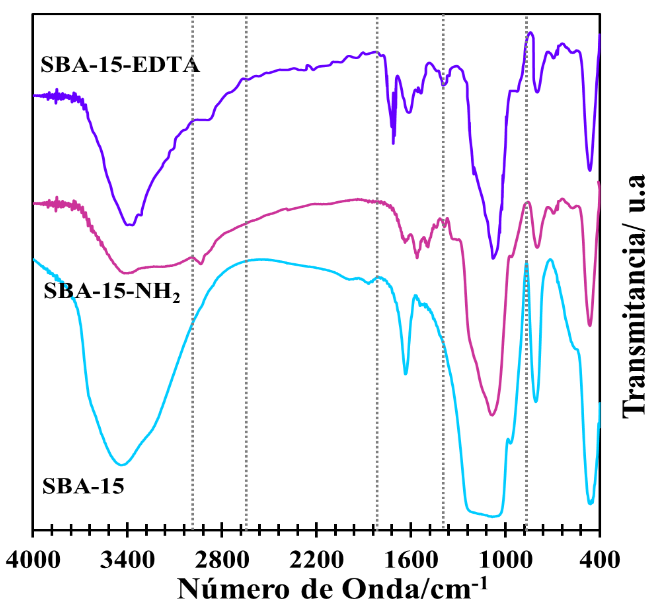
\includegraphics[width=\linewidth]{../structures/IR.png}
				\caption{FTIR}
			\end{figure}
		\end{column}
	\end{columns}
	\footfullcitenomark{melendez_murillo_ramirez_2016}
	\footfullcitenomark{rodriguez}
\end{frame}

\begin{frame}{Discusi\'on}
	\textbf{Hidr\'olisis del \'eter de sililo}
	\begin{figure}[h]
		\centering
		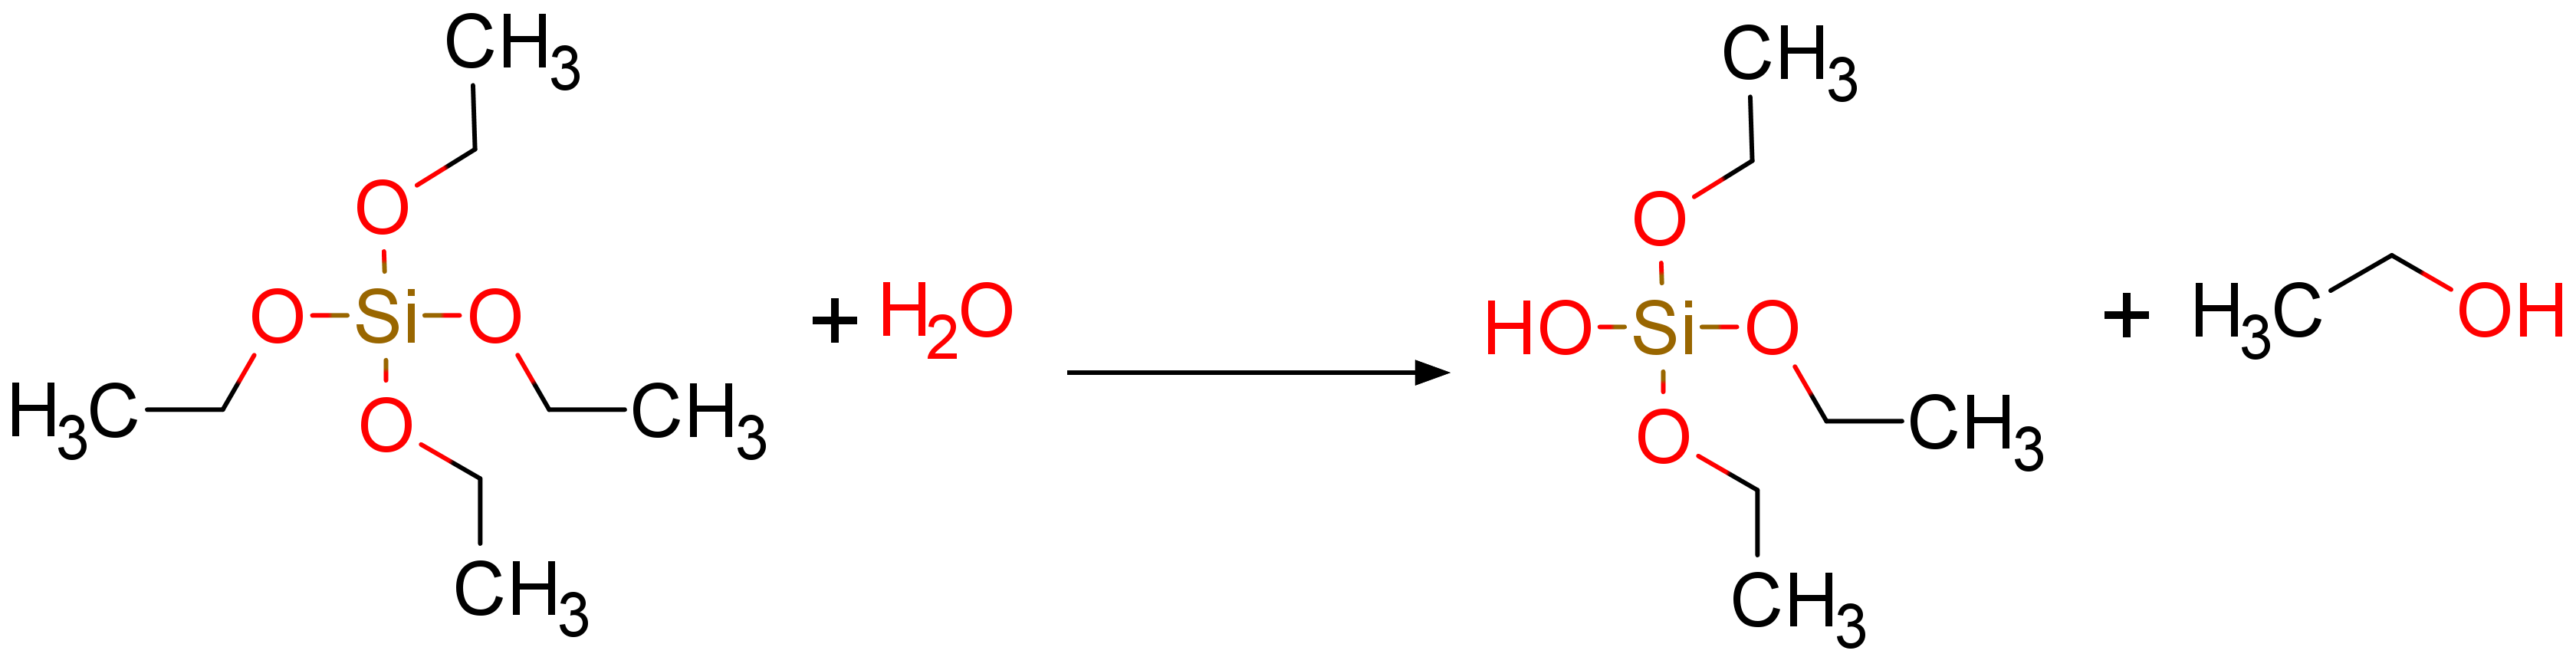
\includegraphics[width = 0.6\linewidth]{../structures/hidrosilicate.png}
	\end{figure}
	\textbf{Condensaci\'on}
	\begin{figure}[h]
		\centering
		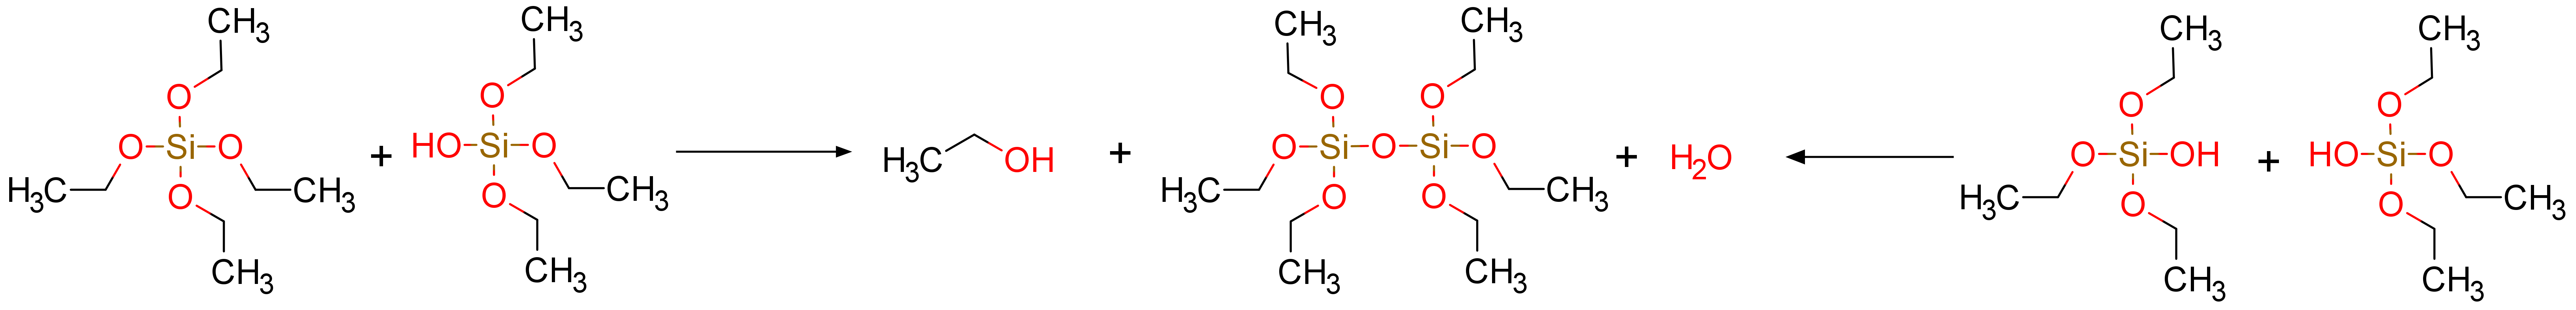
\includegraphics[width = \linewidth]{../structures/polysilicate.png}
	\end{figure}
\end{frame}

\begin{frame}{Discusi\'on}
	\textbf{Formaci\'on de las micelas}
	\begin{figure}[h]
		\centering
		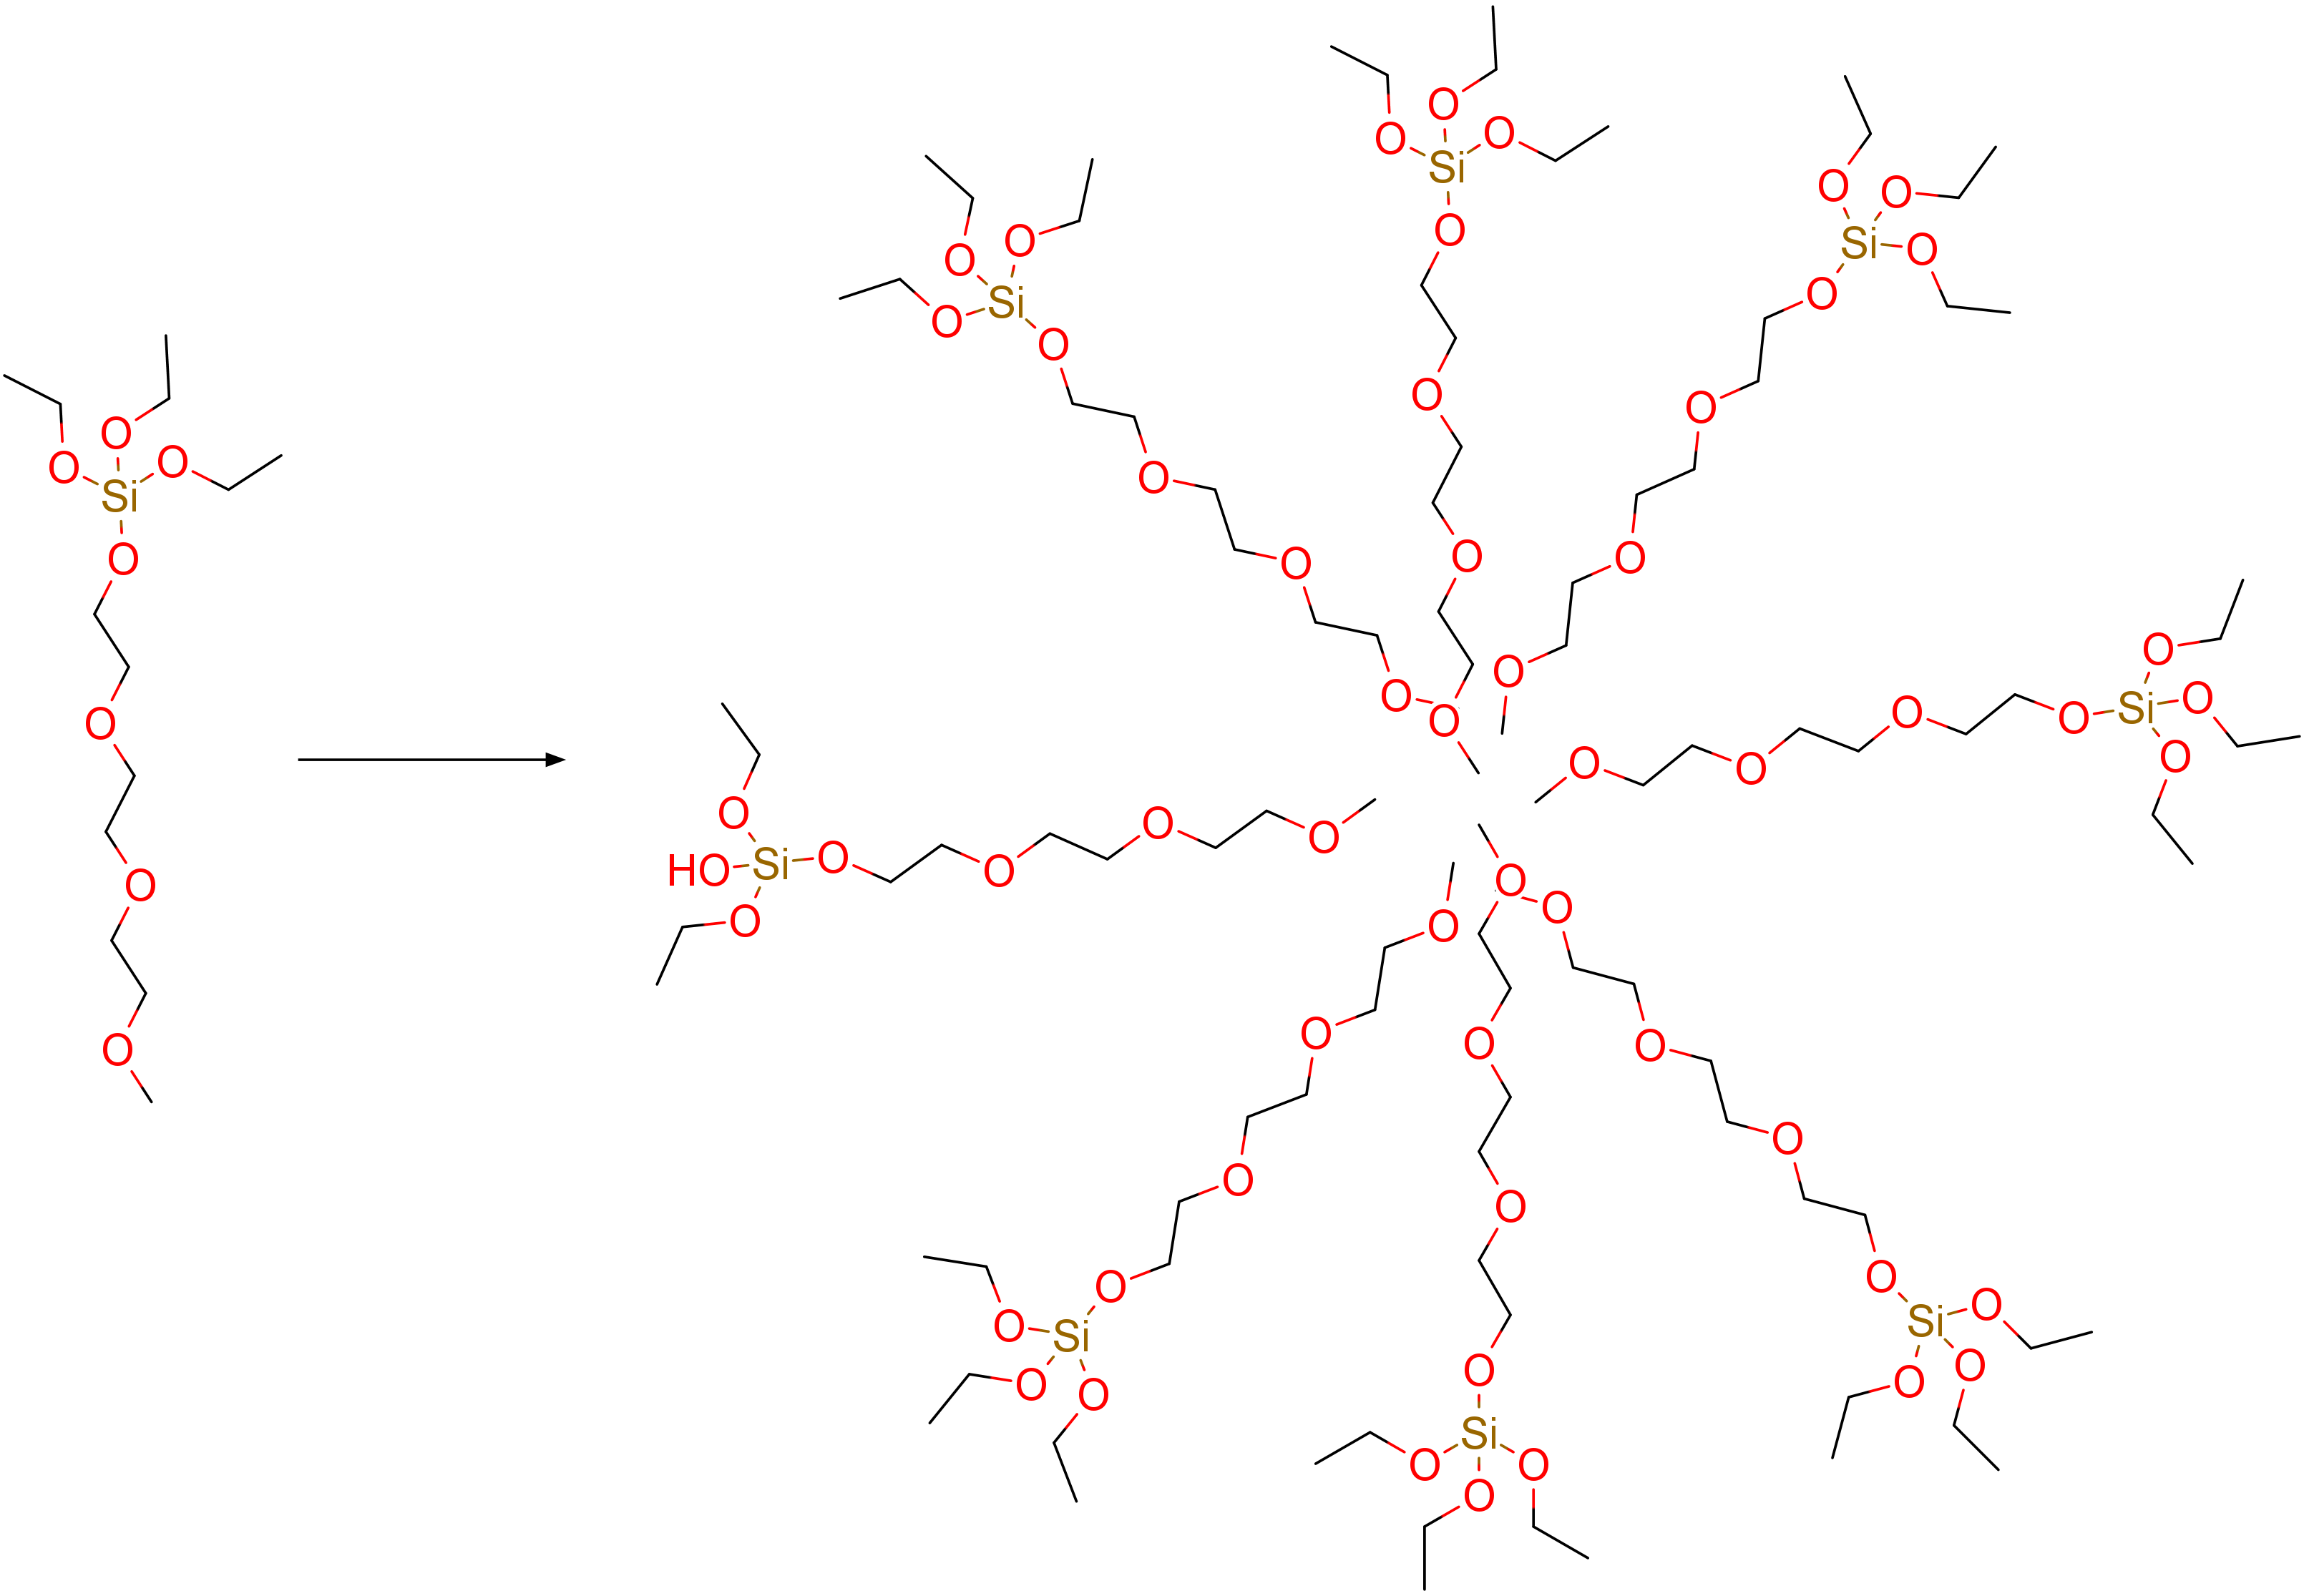
\includegraphics[width = 0.3\linewidth]{../structures/micelaSi.png}
	\end{figure}
	\textbf{Formaci\'on del caparaz\'on de silanol.}
	\begin{columns}
		\begin{column}{0.5\textwidth}
			\begin{figure}[h]
				\centering
				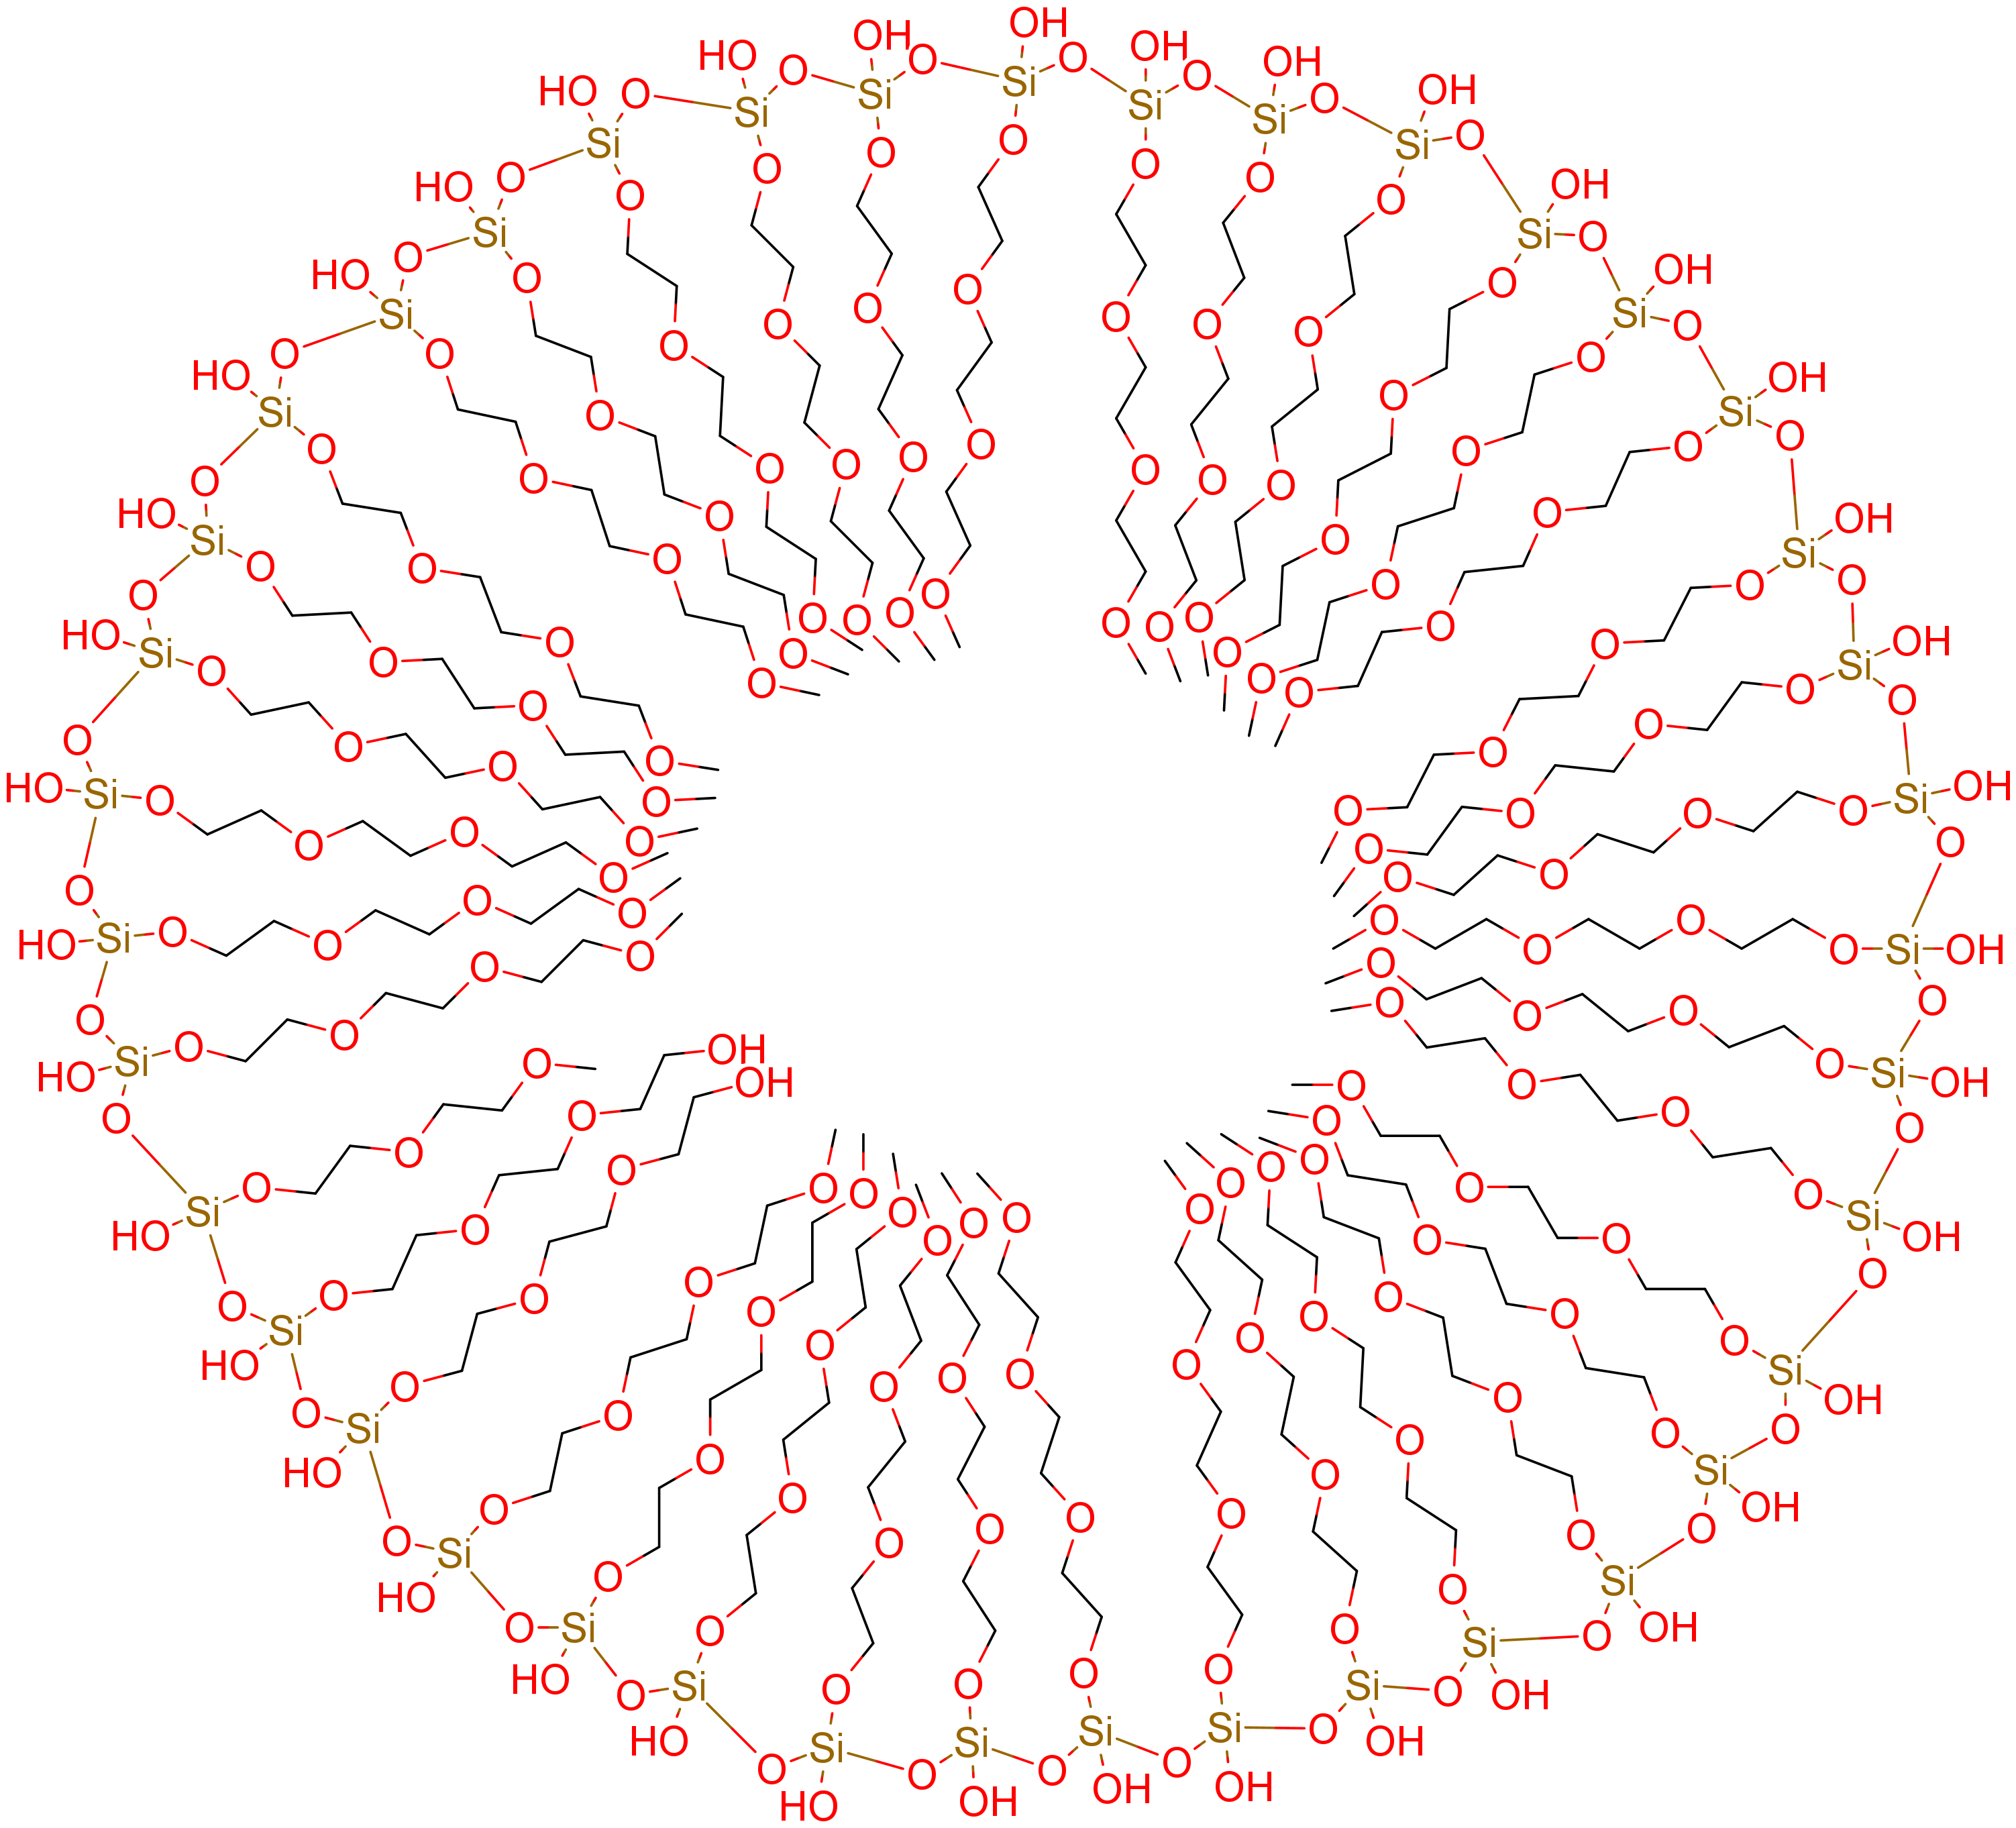
\includegraphics[width = 0.8\linewidth]{../structures/micelaSi2.png}
			\end{figure}
		\end{column}
		\begin{column}{0.5\textwidth}
			\begin{figure}[h]
				\centering
				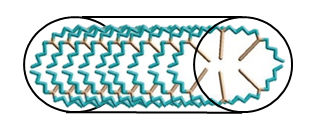
\includegraphics[width = 0.8\linewidth]{../structures/micela3D.png}
			\end{figure}
		\end{column}
	\end{columns}
\end{frame}

\begin{frame}{Conclusiones}
	\begin{itemize}
		\item Fue posible obtener un s\'olido blanco, y muy fino.
		\item Los an\'alisis termogravim\'etricos, y de infrarrojo muestran el acoplamiento del APTES a la estructura del SBA-15.
	\end{itemize}
\end{frame}
\end{document}